% ===================================================================
\section{Competition and invasions (EE04)}
% ===================================================================

\subsection{What competition is}
\textbf{Competition}: any use or defence of a resource by one individual that reduces its availability to others.
\begin{itemize}
\item \textbf{Intraspecific}: within a species. The density-dependent fall of growth in EE03 ($r'=r(1-N/K)$) is
intraspecific competition; so is competition for mates.
\item \textbf{Interspecific}: two species competing for the same \emph{limiting} resource. Two defining features: it is
\textbf{non-trophic} (neither eats the other), and it \textbf{reduces the growth rate or equilibrium number of at
least one} of them. If the species do not affect each other, there is no competition.
\end{itemize}
Exploitation (using the resource up) and interference (blocking access) are both competition; the models here are
about exploitation. Competing is not fighting: two shops on a street compete for a limited pool of customers whether
or not the owners ever meet.

\subsection{Competitive exclusion and the $R^*$ rule}
\textbf{Gause}: \emph{Paramecium aurelia} and \emph{P.\ caudatum} each reach a carrying capacity alone; together,
\emph{P.\ aurelia} keeps increasing and \emph{P.\ caudatum} declines. \textbf{Competitive exclusion principle}: ``no
two species with the same niche can coexist''. \textbf{Tilman (1981)}: diatoms competing for silicate; ``two species
cannot coexist on a single limiting resource''. (Slide 8 notes the original figure's legend should be inverted; do
not quote the winner from the colours.)

\begin{chain}[: why the lowest $R^*$ wins]
\begin{enumerate}
\item Species $i$ grows at per-capita rate $f_i(R)-m_i$, where $f_i$ rises with resource level $R$ and $m_i$ is its
loss rate. It can grow only while $R>R^*_i$, the break-even level where $f_i(R^*_i)=m_i$.
\item Alone, each species draws $R$ down to its own $R^*$ and stops there.
\item Together, with $R^*_1<R^*_2$: species 1 keeps pushing $R$ down towards $R^*_1$. At any $R<R^*_2$ species 2's
growth is negative \emph{even though it is still eating}. So species 2 cannot persist.
\item Therefore the winner is the species that can maintain positive growth at the lowest resource level, not the one
that grows fastest when food is plentiful. With a Monod response $f=\mu R/(k+R)$: $R^*=mk/(\mu-m)$.
\end{enumerate}
\end{chain}

\begin{worked}[: the fast grower loses]
$m=0.2$. A: $\mu=0.8$, $k=2$, $R^*_A=0.667$. B: $\mu=0.6$, $k=1$, $R^*_B=0.5$. At $R=10$, A grows faster (0.667 vs
0.545). But B draws $R$ down to 0.5, where A's growth is $0.16<0.2$: A goes extinct. And adding food to help the loser
does not change either $R^*$, so it does not change the winner, only the winner's numbers.
\end{worked}

\subsection{The Lotka--Volterra competition model}
\[
\frac{\dd N_1}{\dd t}=\frac{r_1N_1(K_1-N_1-\alpha_{12}N_2)}{K_1},\qquad
\frac{\dd N_2}{\dd t}=\frac{r_2N_2(K_2-N_2-\alpha_{21}N_1)}{K_2}.
\]
$\alpha_{12}$ is the effect of one individual of species \textbf{2 on species 1}, measured in \emph{intraspecific
equivalents}: $\alpha_{12}=3$ means one individual of species 2 suppresses species 1 as much as three of its own;
$\alpha_{12}=0$, no effect; $\alpha_{12}=1$, ecological equivalents.

\textbf{Isoclines} (zero growth): species 1: $N_1=K_1-\alpha_{12}N_2$ (intercepts $K_1$ on the $N_1$ axis,
$K_1/\alpha_{12}$ on the $N_2$ axis); species 2: $N_2=K_2-\alpha_{21}N_1$ (intercepts $K_2$ and $K_2/\alpha_{21}$). Species 1
grows when $N_1+\alpha_{12}N_2<K_1$: the crowding it feels (own numbers plus competitors in its own units) is below what
it tolerates. So each species increases below (inside) its isocline and decreases above it.

\begin{center}
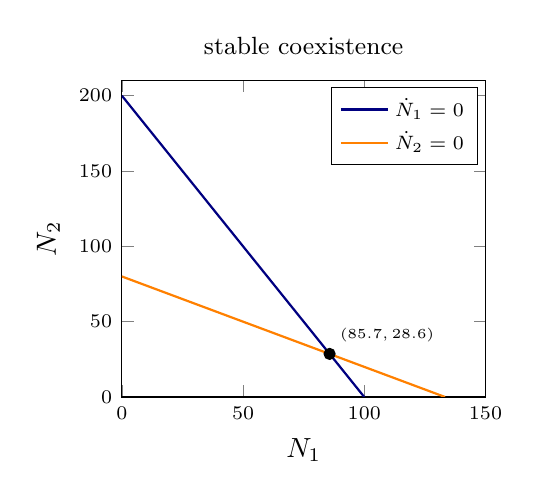
\begin{tikzpicture}
\begin{axis}[width=6.2cm,height=5.6cm,xlabel={$N_1$},ylabel={$N_2$},xmin=0,xmax=150,ymin=0,ymax=210,
  title={\small stable coexistence},tick label style={font=\scriptsize},
  legend style={font=\scriptsize,at={(0.98,0.98)},anchor=north east}]
\addplot[thick,NavyBlue] coordinates {(100,0)(0,200)}; \addlegendentry{$\dot N_1=0$}
\addplot[thick,orange] coordinates {(0,80)(133.3,0)}; \addlegendentry{$\dot N_2=0$}
\addplot[only marks,mark=*] coordinates {(85.7,28.6)};
\node[font=\tiny,anchor=south west] at (axis cs:86,30) {$(85.7,28.6)$};
\end{axis}
\end{tikzpicture}\hspace{3mm}
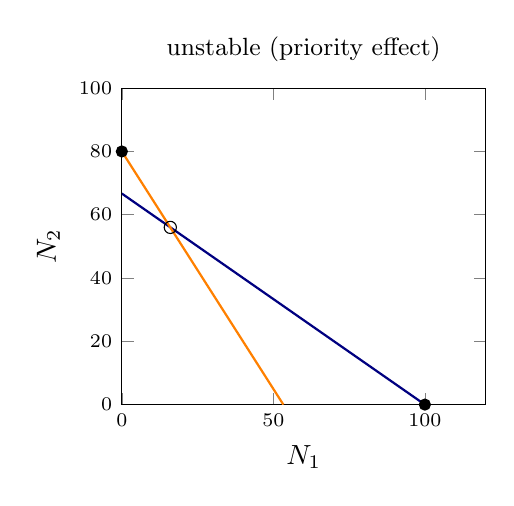
\begin{tikzpicture}
\begin{axis}[width=6.2cm,height=5.6cm,xlabel={$N_1$},ylabel={$N_2$},xmin=0,xmax=120,ymin=0,ymax=100,
  title={\small unstable (priority effect)},tick label style={font=\scriptsize}]
\addplot[thick,NavyBlue] coordinates {(100,0)(0,66.7)};
\addplot[thick,orange] coordinates {(0,80)(53.3,0)};
\addplot[only marks,mark=o,mark size=2.2pt] coordinates {(16,56)};
\addplot[only marks,mark=*] coordinates {(100,0)(0,80)};
\end{axis}
\end{tikzpicture}

\small $K_1=100$, $K_2=80$. Left: $\alpha_{12}=0.5$, $\alpha_{21}=0.6$. Right: $\alpha_{12}=\alpha_{21}=1.5$; filled dots stable,
open dot a saddle.
\end{center}

\begin{chain}[: the four outcomes as two invasion tests]
Ask: can a species increase when \emph{rare}, with the other sitting at its own $K$?
\begin{itemize}
\item Can 2 invade 1? Rare species 2 feels crowding $\alpha_{21}K_1$, so it grows iff $\alpha_{21}K_1<K_2$, i.e.\ $K_1<K_2/\alpha_{21}$.
\item Can 1 invade 2? Iff $\alpha_{12}K_2<K_1$, i.e.\ $K_2<K_1/\alpha_{12}$.
\end{itemize}
\begin{center}\small
\begin{tabular}{lll}
\toprule
1 invades 2? & 2 invades 1? & outcome\\\midrule
yes & no & species 1 wins\\
no & yes & species 2 wins\\
yes & yes & \textbf{stable coexistence} (whoever becomes rare grows back)\\
no & no & \textbf{unstable equilibrium}: priority effect, the start decides\\\bottomrule
\end{tabular}
\end{center}
Coexistence therefore requires $\alpha_{12}<K_1/K_2$ \emph{and} $\alpha_{21}<K_2/K_1$: \textbf{each species limits itself
more than it limits the other}. Slide 12: in 3 of the 4 cases one species drives the other extinct.
\end{chain}

At a coexistence point, $N_1^*=\dfrac{K_1-\alpha_{12}K_2}{1-\alpha_{12}\alpha_{21}}$,
$N_2^*=\dfrac{K_2-\alpha_{21}K_1}{1-\alpha_{12}\alpha_{21}}$, each below its own $K$. The Jacobian determinant is
proportional to $1-\alpha_{12}\alpha_{21}$, so an interior point that \emph{exists} is stable iff $\alpha_{12}\alpha_{21}<1$.

\begin{trap}
\begin{itemize}
\item Index order: $\alpha_{12}$ is the effect of 2 \emph{on} 1. Swapping it swaps the isoclines.
\item $\alpha_{12}\alpha_{21}<1$ is necessary, not sufficient: with unequal $K$ the interior point may not exist
(e.g.\ $\alpha_{21}K_1>K_2$ gives $N_2^*<0$). Check both invasion conditions.
\item $\alpha>1$ does not by itself mean exclusion, if $K_1/K_2$ is large enough.
\item ``3 of 4 outcomes are exclusion'' is a statement about the model's regions, not a claim that exclusion is common in
nature.
\end{itemize}
\end{trap}

\begin{worked}[: 2025 mid-sem Q11]
$K_1=250$, $\alpha_{12}=1.4$; $K_2=1500$, $\alpha_{21}=0.9$. Species 1's isocline runs $(250,0)$--$(0,178.6)$; species 2's
runs $(1667,0)$--$(0,1500)$. Species 2's line lies outside species 1's on both axes, so \textbf{species 2 wins} from any
start, ending at $(0,1500)$. ($r$ values do not affect the outcome, only the speed.)
\end{worked}

\subsection{Invasive species: super-competitors}
An invader arriving without its natural enemies and with efficient resource use acts like a species with large
$\alpha_{\text{inv}\to\text{nat}}$ and small $\alpha_{\text{nat}\to\text{inv}}$: the ``invader wins'' region.
\textbf{Kerala}: the 2018--2019 floods released aquaculture and aquarium fish (arapaima, up to 200\,kg; alligator gar, up to
137\,kg). A 2021 survey of 44 rivers and 53 reservoirs found \textbf{28 alien fish and 4 alien aquatic weeds, 7
established}; main routes: aquarium trade and aquaculture. Water hyacinth (also in the Mula river at Dapodi, per the
wrap-up lecture) is turned into crafts and sarees in Kerala, Assam and West Bengal. Self-study: Asian carps,
\emph{Caulerpa taxifolia}.

Competition is only one mechanism of invasion success: propagule pressure, disturbance, and demographic and genetic
accidents of small founding groups (bottlenecks, inbreeding) also matter; that is why most introductions fail
(background: Sakai et al.\ 2001).

\subsection{Why similar species coexist: the niche and its partitioning}
The \textbf{niche} is an $n$-dimensional hypervolume of conditions and resources. Two meanings:
\begin{itemize}
\item \textbf{Population-persistence niche} (Hutchinson): the range of conditions that allow a population to persist
(positive growth rate) in a place: \emph{where it can live}.
\item \textbf{Resource-utilisation niche} (MacArthur, Levins): what members of the population actually do, in particular
how they use resources: \emph{what it does}.
\end{itemize}
\textbf{Fundamental} niche: where a species could persist without enemies and competitors; \textbf{realised} niche:
where it actually does. Partitioning lowers overlap and so lowers $\alpha$ until the coexistence conditions hold: it
changes the parameters, not the model.

\begin{center}\small
\begin{tabularx}{\textwidth}{lX}
\toprule
type & case and logic\\\midrule
spatial & Gause: \emph{P.\ caudatum} feeds in the top layer, \emph{P.\ bursaria} at the bottom; they coexist.\\
spatial & Connell's barnacles: \emph{Chthamalus} high on the shore (\emph{Balanus} desiccates there); \emph{Balanus} in the
middle, where it outcompetes \emph{Chthamalus} for space; lower, \emph{Balanus} suffers predation. Physical limits set
the upper edge of one species, competition the lower edge of the other: realised $<$ fundamental.\\
temporal & Spiny mice in Israel: common (\emph{Acomys cahirinus}) nocturnal, golden (\emph{A.\ russatus}) diurnal. Remove the
common species and the golden one becomes nocturnal: the separation is \emph{induced} by competition.\\
morphological & Character displacement: traits of related species differ \emph{more where they co-occur} than where
they are apart (beak depths of Galápagos ground finches on different islands).\\
conditional & Park's \emph{Tribolium}: \emph{confusum} wins cool-dry (100\,\%), \emph{castaneum} wins warm-moist (100\,\%).\\\bottomrule
\end{tabularx}
\end{center}

\begin{keyidea}[: Park's lesson]
A higher single-species equilibrium does \emph{not} guarantee victory. Cool-moist: \emph{castaneum} is larger alone
(45.2 vs 28.2) yet loses 71\,\% of contests; warm-moist: \emph{confusum} is larger (41.2 vs 38.3) and loses every
contest. $K$ is half the story; the competition coefficients, which change with temperature and humidity, decide the
contest. If conditions switch faster than exclusion takes, neither wins permanently.
\end{keyidea}

\begin{statements}
\begin{enumerate}[label=\arabic*.]
\item ``A lion eating a zebra is an extreme form of interspecific competition.''
\F Competition is non-trophic; eating is predation.
\item ``The species with the highest growth rate at high resource density wins exploitative competition.''
\F The species with the lowest $R^*$ wins; the fast grower at high food can lose.
\item ``If $\alpha_{12}\alpha_{21}<1$, the two species must coexist.''
\F Necessary for a stable interior point but not sufficient; with unequal $K$, check $\alpha_{12}<K_1/K_2$ and $\alpha_{21}<K_2/K_1$.
\item ``In the unstable-equilibrium case, the winner is decided by the starting numbers.''
\T Neither can invade the other; the saddle's separatrix splits the plane (priority effect, a kind of bistability).
\item ``The golden spiny mouse is diurnal because diurnality is in its fundamental niche only.''
\F It becomes nocturnal when the competitor is removed: diurnality is its \emph{realised} niche, induced by competition.
\item ``Character displacement predicts that two related species are \emph{more} similar where they co-occur.''
\F More \emph{different} where they co-occur.
\item ``Coexisting competitors probably partition the niche, though showing how is often hard.''
\T This is the wrap-up lecture's own summary for competition.
\item ``Feeding an endangered native fish more will help it against an invader limited by the same single food.''
\F Feeding raises supply but leaves both $R^*$ unchanged; the invader still draws food down below the native's break-even.
\end{enumerate}
\end{statements}

\begin{longans}[: ``In 3 of 4 cases L--V competition predicts exclusion, yet many similar species coexist. Resolve.'']
(1) Model, isoclines, the four outcomes via invasion tests; coexistence iff each limits itself more than the other.
(2) Exclusion seen in simple lab settings: Gause (\emph{aurelia} vs \emph{caudatum}), Tilman (one resource), $R^*$.
(3) Mechanism 1, niche partitioning lowers $\alpha$: spatial (\emph{caudatum}/\emph{bursaria}; barnacles), temporal
(spiny mice removal), morphological (character displacement). (4) Mechanism 2, conditional outcomes and fluctuating
environments: Park's \emph{Tribolium}. (5) The model gives a precise question; experiments find which condition holds.
\end{longans}
